\subsection{Vektorer}

En vektor er en matrix, som enten kun har en sølje eller en række. En vektor med kun en søjle kaldes en søjlevektor, mens en vektor men kun en række kaldes en rækkevektor.
Vektorer anvendes blandt andet til at repræsentere  rækker og søjler i matricer. I dette tilfælde er vektorerne derved delmatricer af den originale matrix.
Indgangene i en vektor kaldes vektorens vektorkomponenter



\begin{defn}[Søjlevektor]
Lad $\underset{m \times n}{A}$ være en matrix, så vil en \textbf{søjlevektor} være en delmatrix med kun en søjle og alle søjlens rækkekomponenter
\begin{align*}
\underset{m \times 1}{A} = 
\begin{bmatrix}
a_{1,i}\\
a_{2,i}\\
\vdots \\
a_{m-1,i}\\
a_{m,i} \\
\end{bmatrix}\qquad , i\in [1,n]%|n\neq1
\end{align*}
\end{defn}

\begin{defn}[Rækkevektor]
Lad $\underset{m \times n}{A}$ være en matrix, så vil en \textbf{rækkevektor} være en delmatrix med kun en række og alle rækkens søjlekomponenter
%En \textbf{Række vektor} er en matrice med 1 række og n søjler
\begin{align*}
\underset{1 \times n}{A} = 
\rvect{a_{j,1} & a_{j,2} & \dots & a_{j,n-1} & a_{j,n}}
\qquad , j\in [1,m]%|m\neq1
\end{align*}
\end{defn}
Bemærk at hvis henholdsvis $m$ eller $n$ er $1$, så er matricen i forvejen en vektor.\\
\\
Addition af to vektorer kan repræsenteres grafisk med pile, ved at tage to ikke-nul vektorer $\vec{u}$ og $\vec{v}$ og forme et parallelogram med vektorene som parallelogrammets sider. I følge parallelogram loven vil diagonalen af parallelogrammet være de to vektor lagt sammen $\vec{u}+\vec{v}$.
%Mangler firgur 1.3 fra lial bogen
\begin{defn}[Addition af to vektor]
Lad $\underset{m \times 1}{A}$ og $\underset{m \times 1}{B}$ være to vektorer med samme størrelse. Da vil additionen af de to vektorer give en vektor, $\underset{m \times 1}{C}$, hvor hver komponent er summen af de tilsvarende komponenter i $\underset{m \times 1}{A}$ og $\underset{m \times 1}{B}$.
\begin{align*}
\underset{m \times 1}{A} = 
\begin{bmatrix}
a_{1,1}\\
a_{2,1}\\
\vdots \\
a_{m-1,1}\\
a_{m,1} \\
\end{bmatrix}
\qquad
\underset{m \times 1}{B} = 
\begin{bmatrix}
b_{1,1}\\
b_{2,1}\\
\vdots \\
b_{m-1,1}\\
b_{m,1} \\
\end{bmatrix}
\end{align*} 
\begin{align*}
C=A+B=
\begin{bmatrix}
a_{1,1}\\
a_{2,1}\\
\vdots \\
a_{m-1,1}\\
a_{m,1} \\
\end{bmatrix}
+
\begin{bmatrix}
b_{1,1}\\
b_{2,1}\\
\vdots \\
b_{m-1,1}\\
b_{m,1} \\
\end{bmatrix}
=
\begin{bmatrix}
a_{1,1}+b_{1,1}\\
a_{2,1}+b_{2,1}\\
\vdots \\
a_{m-1,1}+b_{m-1,1}\\
a_{m,1}+b_{m,1} \\
\end{bmatrix}
\end{align*}
\end{defn}
\begin{eks}
\begin{align*}
A=
\begin{bmatrix}
4\\
1\\
0\\
-5\\
\end{bmatrix}
\hspace{3cm}
B=
\begin{bmatrix}
7\\
4\\
-2\\
-5\\
\end{bmatrix}\\
A+B=
\begin{bmatrix}
4\\
1\\
0\\
-5\\
\end{bmatrix}
+
\begin{bmatrix}
7\\
4\\
-2\\
-4\\
\end{bmatrix}
=
\begin{bmatrix}
4+7\\
1+4\\
0-2\\
-5-4\\
\end{bmatrix}
=
\begin{bmatrix}
11\\
5\\
-2\\
-9\\
\end{bmatrix}
\end{align*}
\end{eks}

Hvis en vektor kan lægges til en anden vektor, så må det også være muligt at skalere den. Det vil sige multiplicere den med en konstant, eftersom $2\vec{x}=\vec{x}+\vec{x}$.\\  %giver god mening, men det lyder som et bevis
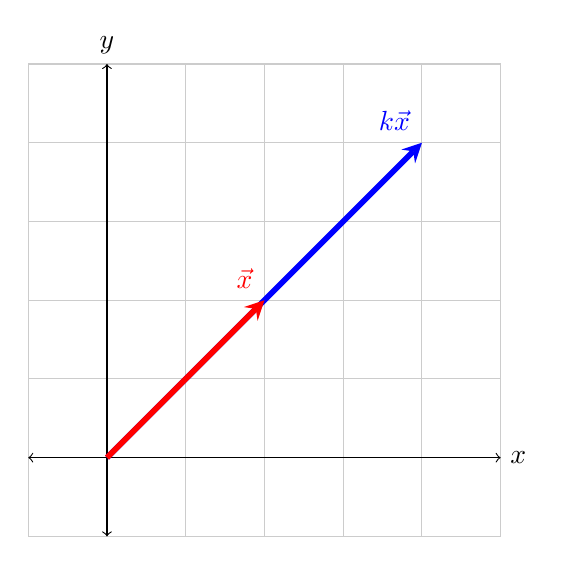
\begin{tikzpicture}
  \draw[thin,gray!40] (-1,-1) grid (5,5); %laver Grid
  \draw[<->] (-1,0)--(5,0) node[right]{$x$}; %x-aksen
  \draw[<->] (0,-1)--(0,5) node[above]{$y$}; %y-aksen
  \draw[line width=2pt,blue,-stealth](0,0)--(4,4) node[above left]{$k\vec{x}$}; %blå vektor
  \draw[line width=2pt,red,-stealth](0,0)--(2,2) node[above left]{$\vec{x}$}; %rød vektor
\end{tikzpicture}
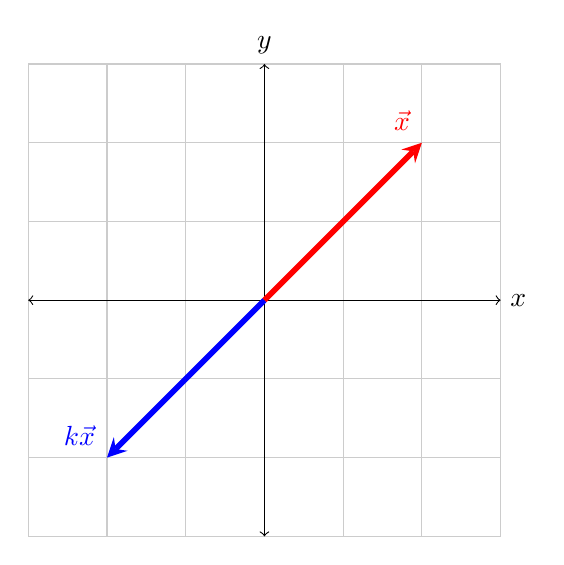
\begin{tikzpicture}
  \draw[thin,gray!40] (-3,-3) grid (3,3);
  \draw[<->] (-3,0)--(3,0) node[right]{$x$};
  \draw[<->] (0,-3)--(0,3) node[above]{$y$};
  \draw[line width=2pt,blue,-stealth](0,0)--(-2,-2) node[above left]{$k\vec{x}$};
  \draw[line width=2pt,red,-stealth](0,0)--(2,2) node[above left]{$\vec{x}$};
\end{tikzpicture}
\begin{defn}[Vektor skalar]
Lad $\vec{x}$ være en vektor i $\mathds{R}^n$. Da er et \textbf{Vektor skalar} produktet af den vektorens komponenter multipliceret med konstanten.
%En \textbf{Vektor skalar} er produktet af en vektor $\vec{x}$
%som bliver multipliceret med en konstant $k$ kaldet skalar. Denne vektor peger i samme retning, men har en anden længde.
\begin{align*}
\vec{x}=\begin{bmatrix}
x_1\\
x_2\\
\vdots\\
x_{n-1}\\
x_n
\end{bmatrix}\\
k\vec{x}=k\begin{bmatrix}
x_1\\
x_2\\
\vdots\\
x_{n-1}\\
\end{bmatrix}=
\begin{bmatrix}
kx_1\\
kx_2\\
\vdots\\
kx_{n-1}\\
kx_n\\
\end{bmatrix}
\end{align*}
\end{defn}
\begin{eks}
En vektor $\vec{x}$ med komponenterne $2$ og $3$ skal skaleres med konstanten $k=3$, hvilket gøres ved at multiplicere konstanten med begge komponenter.
\begin{align*}
\vec{x}=\begin{bmatrix}
2\\
3
\end{bmatrix}\qquad k=3\\
k\vec{x}=3
\begin{bmatrix}
2\\
3
\end{bmatrix}
=
\begin{bmatrix}
3\cdot2\\
3\cdot3
\end{bmatrix}
=
\begin{bmatrix}
6\\
9
\end{bmatrix}
\end{align*}
\end{eks}
\subsection{Matrix-vector produkt}
Et matrix-vektor produkt, er produktet af en $m\times n$ matrix og en vektor. Dette lægger grundlaget for hvordan matricer ganges sammen, eftersom en vektor også kan ses som en $n\times1$ matrix. 
\begin{defn}[Matrix-vektor produkt]
Lad $A$ være en $mxn$ matrix og $x$ være en $mx1$ vektor. Så skrives \textbf{Matrix-vektor produktet} $A\vec{x}$, som produktet af søjlerne $\vec{A_j}$ i $A$ og de tilsvarende komponenter i $\vec{x}$. Dette kræver at matricen har samme antal søjler som vektoren har komponenter, hvilket er defineret med $n$.
\begin{align*}
A\vec{x}&=x_1\vec{A}_1+x_2\vec{A}_2+ \dots +x_{n-1}\vec{A}_{n-1}+x_n\vec{A}_n \\
&=
\begin{bmatrix}
x_1a_{1 1}+x_2a_{1 2}+\dots +x_{n-1}a_{1 n-1}+x_na_{1 n} \\
x_1a_{2 1}+x_2a_{2 2}+\dots +x_{n-1}a_{2 n-1}+x_na_{2 n}\\
\vdots\\
x_1a_{m-1 1}+x_2a_{m-1 2}+\dots +x_{n-1}a_{m-1 n-1}+x_na_{m-1 n} \\
x_1a_{m 1}+x_2a_{m 2}+\dots +x_{n-1}a_{m n-1}+x_na_{m n}
\end{bmatrix}
=
\begin{bmatrix}
\vec{a}_1\vec{x}\\
\vec{a}_2\vec{x}\\
\vdots\\
\vec{a}_{m-1}\vec{x}\\
\vec{a}_m\vec{x}
\end{bmatrix}.
\end{align*}
\end{defn}
\begin{eks}
\begin{align*}
A=
\begin{bmatrix}
1 & 4\\
2 & 5\\
3 & 6
\end{bmatrix}
\qquad
\vec{x}=
\begin{bmatrix}
7\\
8
\end{bmatrix} \\
A\vec{x}= \begin{bmatrix}
1 & 4\\
2 & 5\\
3 & 6
\end{bmatrix}
\begin{bmatrix}
7\\
8
\end{bmatrix}
=
7
\begin{bmatrix}
1\\
2\\
3
\end{bmatrix}
+ 8
\begin{bmatrix}
4\\
5\\
6
\end{bmatrix}=
\begin{bmatrix}
7\\
14\\
21
\end{bmatrix}
+
\begin{bmatrix}
32\\
40\\
48
\end{bmatrix}
=
\begin{bmatrix}
39\\
54\\
69
\end{bmatrix}
\end{align*}
\end{eks}
\subsection{Standard basis vektorer}
Standard basis vektorer, er vektorer som har længden $1$ og følger akserne i det rum $\mathds{R}^n$ vektoren er i.\\
Standard basis vektorer i $\mathds{R}^n$ skrives som $e_i$, hvor $i\in[1,n]$ og $i$ er den vektor komponent som har værdien $1$ og resten $0$.

\begin{defn}[Standart basis vektorer]
Lad $e_m$ være en $m\times 1$ vektor i $\mathds{R}^m$ med alle indgange/komponenter $a_i=0$
\begin{align*}
e_i=e_m|a_i\in e_m=1 \forall i\in[1,m] %stadig ikke helt sikker på det, men det giver mere mening
\end{align*}

\end{defn}